\chapter{简介}
复旦大学数学科学学院研究生毕业论文 LaTeX 模版基于开源模版fduthesis开发by 曾祥东\footnote{https://github.com/stone-zeng/fduthesis},我们对他表示感谢。本模板的第一版由复旦大学数学科学学院2021级罗心悦整理完成,目前为迭代的第二版模板,由2019级冯典等在第一版的基础上进行了更新。关于模板更新的内容,我们将在下文详细指出。部分内容摘自复旦大学数学科学学院2023年毕业生邹森博士的毕业论文。说明性文字参考了上海交通大学学位论文模版\footnote{https://github.com/sjtug/SJTUThesis}。 

本模板依然在持续的迭代更新中,计划每年向学院官网\footnote{https://math.fudan.edu.cn/30396/list.htm}提供一次大更新,日常迭代更新的版本请跳转\href{https://github.com/VeMath/fduMath_thesis}{{\color{red} github仓库}}\footnote{https://github.com/VeMath/fduMath\_thesis}。
欢迎大家指出模板的不足之处,有任何意见可以在github仓库中提交issue。对于模版有改进建议,也可直接提交PR。如有其它问题,可联系项目维护人员罗心悦:\href{mailto:xinyueluo21@m.fudan.edu.cn}{xinyueluo21@m.fudan.edu.cn}或张晨阳:\href{mailto:24110180062@m.fudan.edu.cn}{24110180062@m.fudan.edu.cn}。


该模版旨在帮助复旦大学数学科学学院的研究生规范撰写毕业论文,符合学院的格式要求,更多细节可以参考《复旦数学科学学院研究生毕业论文\LaTeX{}模版使用说明》。

\section{更新说明}
这一节将给出与上一节的差别,其中对于模板本身的更改仅需了解。对于论文书写比较关键的更改,我们将会用{\color{blue} 蓝色}进行标注。
\subsection{关于引用}
对于不同的引用格式,可参阅biblatex-gb7714-2015宏包文档\footnote{https://mirrors.ustc.edu.cn/CTAN/macros/latex/contrib/biblatex-contrib/biblatex-gb7714-2015/biblatex-gb7714-2015.pdf},如非上标形式的引用可使用\textbackslash parencite命令。

\begin{figure}
    \centering
    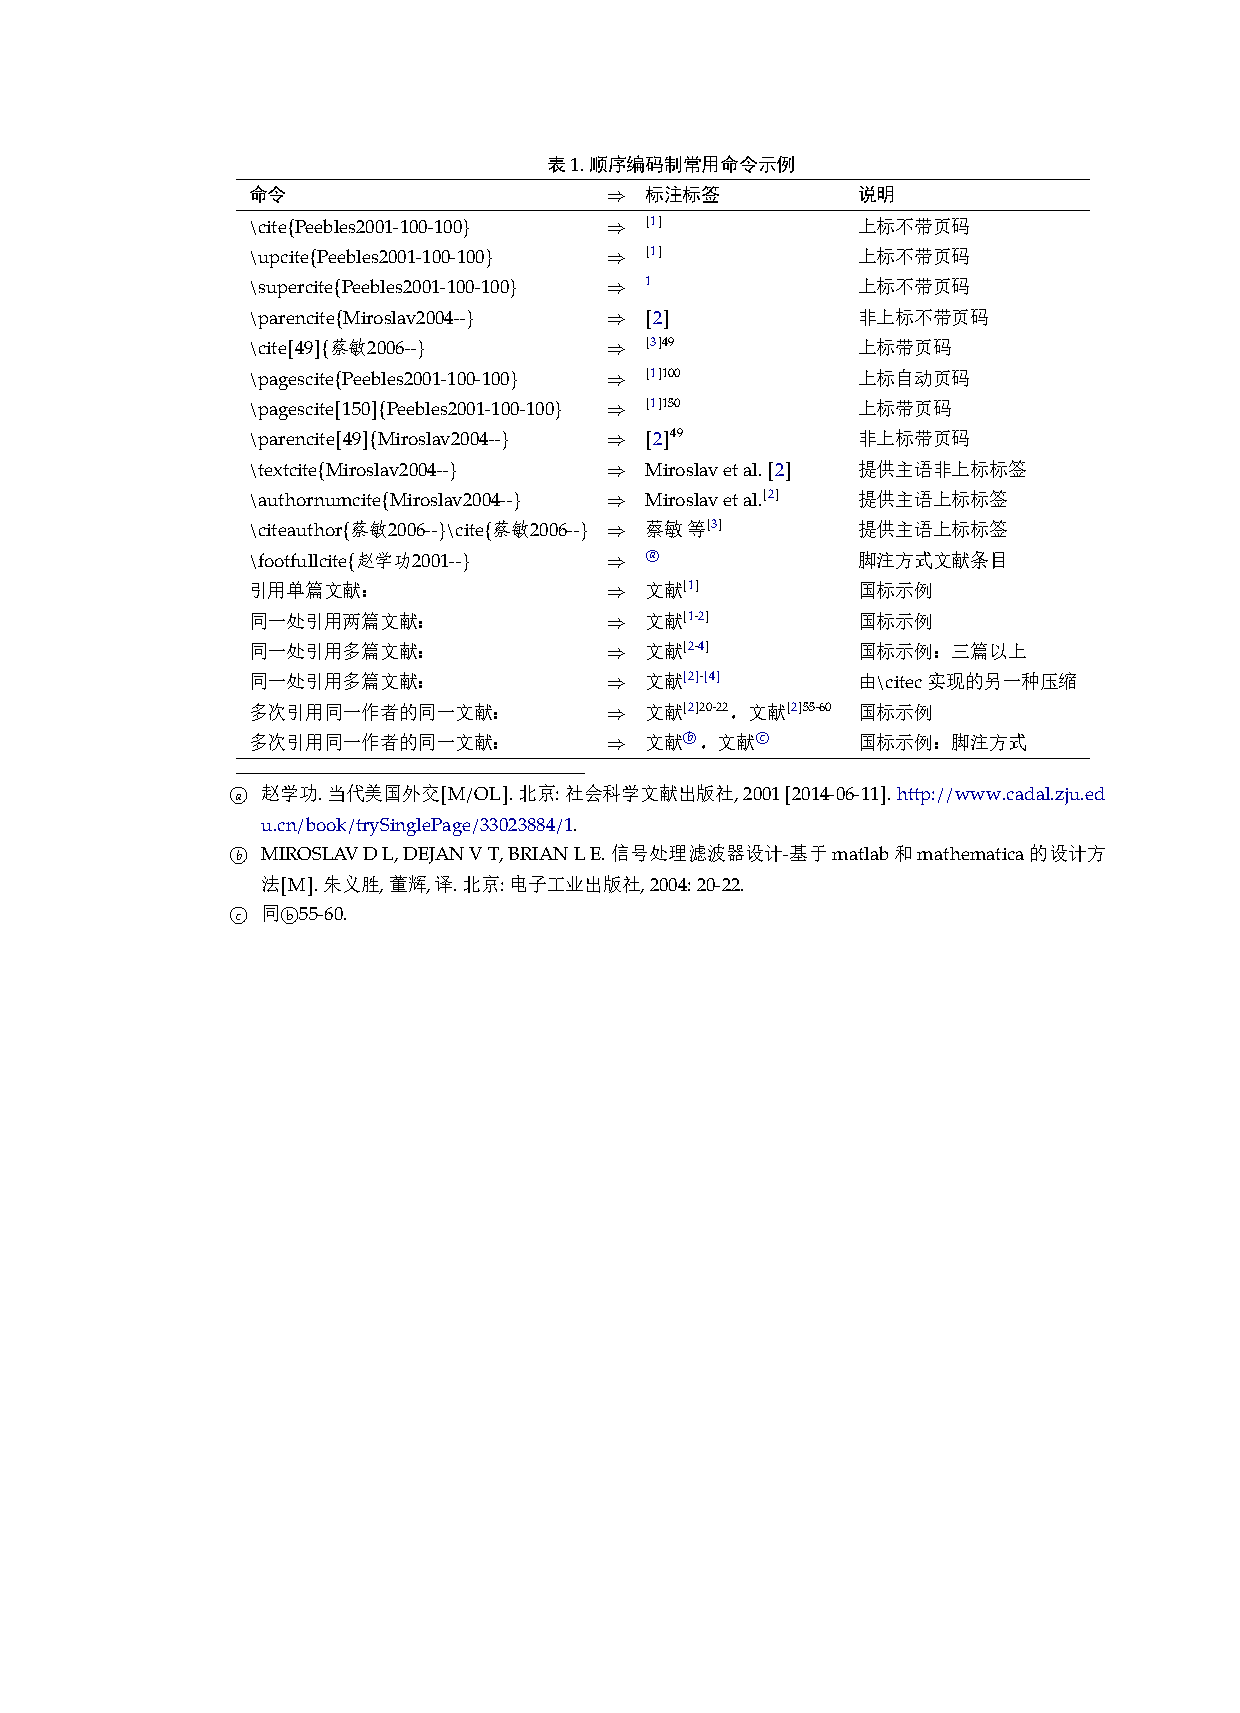
\includegraphics[width=0.8\linewidth]{figs/biblatex-gb7714-2015.pdf}
\end{figure}

\subsection{关于页码位置}

第一版中的页码出现在每一页的正下方,我们对此进行了调整,现在的页码位置分奇偶,奇数页出现在右下角,而偶数页出现在左下角。

目前模板默认的方式是奇数页在右下角,偶数页在左下角。如果确实需要修改回居中格式,可在文件setup.tex中进行修改。
只需将setup.tex中对应代码片段的LE,RO更改为C即可。

奇数页右下角,偶数页左下角:
\begin{codeblock}
\fancyfoot{}
\fancyfoot[EL,OR]{\small\thepage}
\fancypagestyle{plain}{
    \fancyfoot{}
    \fancyfoot[EL,OR]{\small\thepage}
}
\end{codeblock}

页码居中:
\begin{codeblock}
\fancyfoot{}
\fancyfoot[C]{\small\thepage}
\fancypagestyle{plain}{
    \fancyfoot{}
    \fancyfoot[C]{\small\thepage}
}
\end{codeblock}

\subsection{其它调整}
\begin{itemize}
    \item 超链接颜色默认为黑色
    \item 定理、公理、推论等环境默认共享计数器
\end{itemize}
